\section{System model}
\label{sec: system_model}


\begin{figure}[tb]
    \centering
    \scalebox{1.0}{
        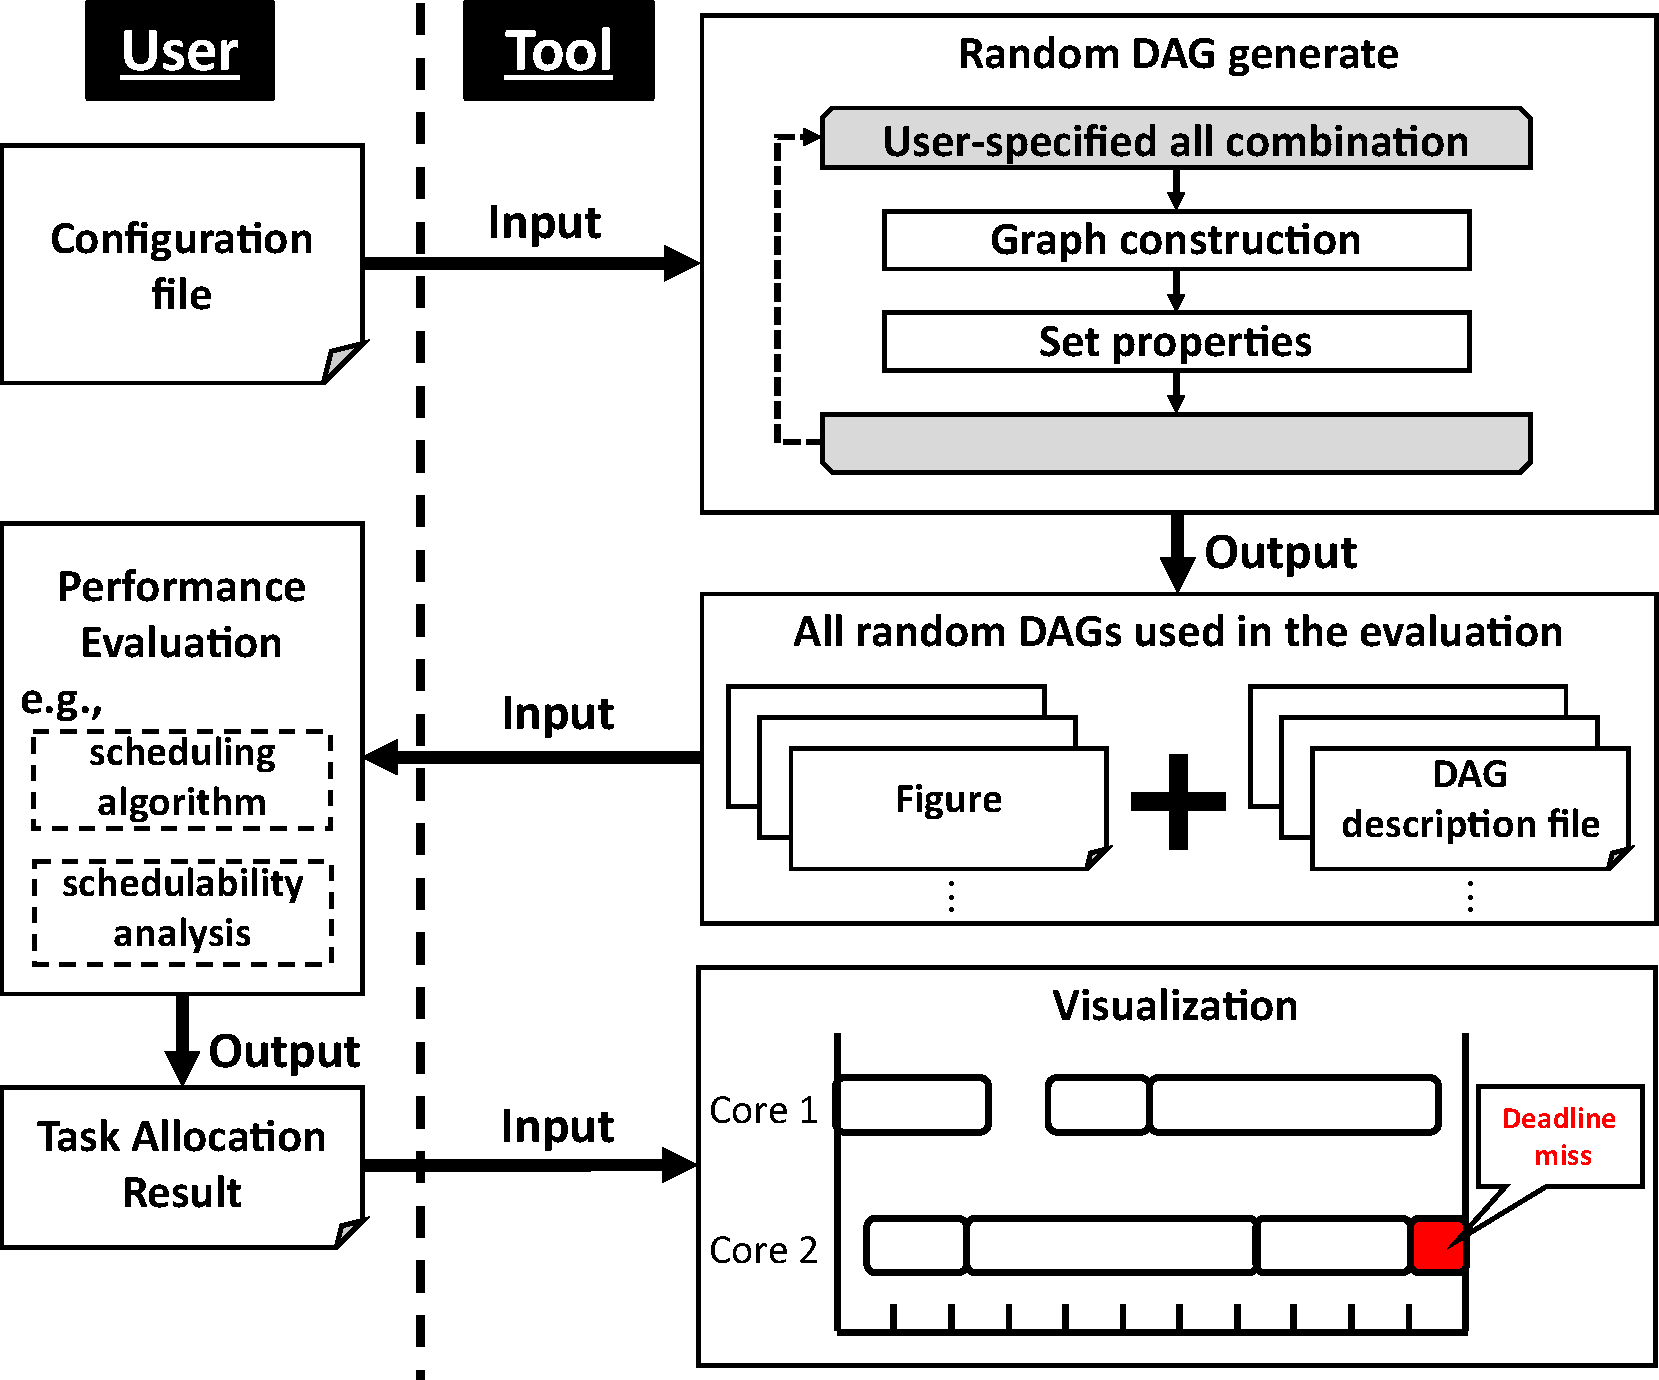
\includegraphics[width=\linewidth]{./src/figure/system_model.pdf}
    }
    \caption{System model.}
    \label{fig: system_model}
\end{figure}


\begin{table}[tb]
    \centering
    \caption{DAG Notations}
    \label{tab: dag_notations}
    \renewcommand{\arraystretch}{1.2}
    \scalebox{1.0}{
        \begin{tabular}{c|l}\hline\hline
            $G$            & DAG                                            \\ \hline
            $V$            & Set of all nodes of $G$                        \\ \hline
            $E$            & Set of all edges of $G$                        \\ \hline
            $\tau_i$       & $i$-th Node                                    \\ \hline
            $C_i$          & WCET of $\tau_i$                               \\ \hline
            $e_{i,j}$      & Edge between $\tau_i$ and $\tau_j$             \\ \hline
            $D$            & End-to-end deadline                            \\ \hline
            $\tau^{tm}_i$  & $i$-th timer-driven node                       \\ \hline
            $\phi_i$       & Offset of $\tau^{tm}_i$                        \\ \hline
            $T_i$          & Execution period of $\tau^{tm}_i$              \\ \hline
            $d_i$          & Relative deadline of $\tau^{tm}_i$             \\ \hline
            $u_i$          & Utilization of $\tau^{tm}_i$                   \\\hline
            $U$            & Total Utilization of $G$                       \\\hline
            $\Gamma_i$     & $i$-th chain                                   \\\hline
            $C_{\Gamma_i}$ & WCET of $\Gamma_i$                             \\ \hline
            $u_{\Gamma_i}$ & Utilization of $\Gamma_i$                      \\ \hline
            $T_{\Gamma_i}$ & Period of head timer-driven node of $\Gamma_i$ \\ \hline
        \end{tabular}
    }
\end{table}


This section represents the system model, as shown in Fig.~\ref{fig: system_model}.
Section~\ref{ssec: single_rate_dag} describes the basic single-rate DAG.
Section~\ref{ssec: multi_rate_dag} explains a multi-rate DAG.
The DAG notations used in this paper are listed in Table~\ref{tab: dag_notations}.


\subsection{Single-rate DAG}
\label{ssec: single_rate_dag}

Single-rate DAGs are DAGs with either a single entry node or all entering at the same time, used in real-time application \cite{zhao2020dag}, cyber-physical systems \cite{senapati2021hmds} and cloud computing \cite{kaur2020deep}, and so forth.
Here, the entry node represents the input to the system (e.g., a sensor event or a command from the user), and the exit node represents the final output from the system.

A DAG consists of a node set and an edge set, denoted $G = (V, E)$.
Nodes represent tasks in the system, and edges represent communication and dependencies between nodes or priority constraints.
$V$ is the set of all nodes, expressed as $V = \{\tau_1, ..., \tau_{|V|}\}$, where $|V|$ is the total number of nodes.
Each node has a worst-case execution time (WCET), and the WCET of $\tau_i$ is denoted as $C_i$.
$E$ is the set of all edges, where each edge $e_{i,j} \in E$ represents communication between $\tau_i$ and $\tau_j$ and a priority constraint.
When $e_{i,j}$ exists in the DAG, $\tau_j$ cannot be executed until $\tau_i$ has completed its execution and the output of $\tau_i$ has arrived.
An end-to-end deadline $D$ is set at the exit node when it is necessary to guarantee the safety of hard real-time systems \cite{yano2021work} or the quality of service of cloud computing \cite{zhang2020efficient}.


\subsection{Multi-rate DAG}
\label{ssec: multi_rate_dag}

A multi-rate DAG is a DAG that contains multiple nodes that are triggered at different periods.
Here, the definitions of nodes and edges in a multi-rate DAG are the same as those shown in Section~\ref{ssec: single_rate_dag}.
Multi-rate DAGs can be broadly classified into two categories: (i) DAGs in which all nodes are timer-driven nodes, as in automotive systems \cite{kordon2020evaluation, verucchi2020latency}, and (ii) DAGs that combine a chain consisting of timer-driven nodes and a chain of linked event-driven nodes, as in self-driving systems \cite{choi2021picas, tang2020response}.


\subsubsection{Multi-rate DAG consisting of only timer-driven nodes}
\label{sssec: dag_only_timer}

Each timer-driven node in these multi-rate DAGs is denoted by $\tau^{tm}_i$, and $\tau^{tm}_i$ is characterized by the tuple $(\phi_i, Ci, Ti, di)$.
$\phi_i$, $T_i$, and $d_i$ represent the offset, execution period, and relative deadline, respectively.
For DAGs that consider timer-driven nodes, every timer-driven node has a relative deadline of $T_i$ time units indicating that every job of $\tau^{tm}_i$ has an absolute deadline at $T_i$ time units after its release \cite{yang2020mixed, cho2021conditionally}.
Such a time constraint is called an implicit deadline, and MRDAG-Gen generates DAGs that consider implicit deadlines.

The utilization of $\tau^{tm}_i$ is denoted as $u_i$ calculated by $u_i = C_i / T_i$.
The total utilization $U$ of a DAG consisting only of timer-driven nodes is defined by Eq.~\ref{eq: total_utilization_only_timer}.

\begin{equation}
    \label{eq: total_utilization_only_timer}
    U = \sum_{\tau^{tm}_i \in V}u_i
\end{equation}


\begin{figure}[tb]
    \centering
    \scalebox{1.0}{
        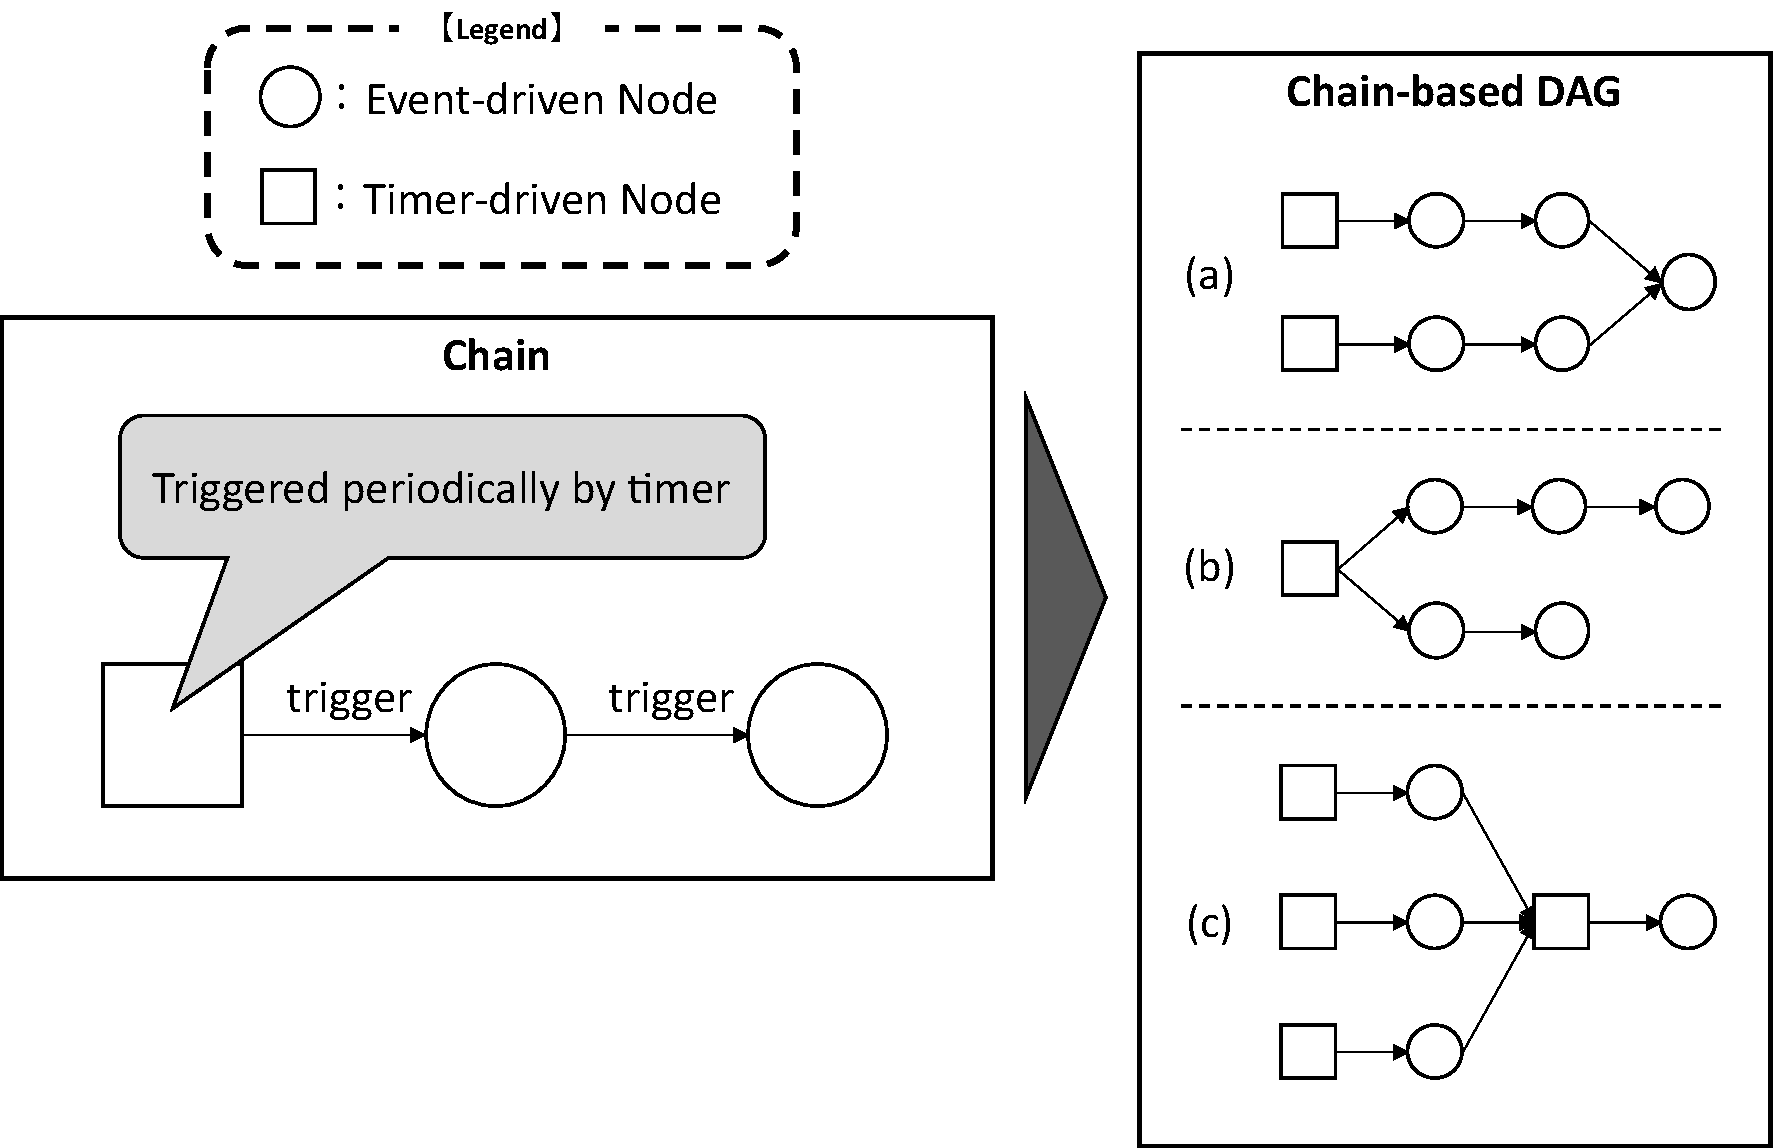
\includegraphics[width=\linewidth]{./src/figure/chain_based_dag.pdf}
    }
    \caption{Multi-rate DAGs consisting of chains}
    \label{fig: chain_dag}
\end{figure}


\subsubsection{Chain-based multi-rate DAG}
\label{sssec: dag_chain}

In the latest multi-rate systems, DAGs consisting of the chain shown in Fig.~\ref{fig: chain_dag} are considered.
Each chain $\Gamma_i$ is denoted as $\Gamma_i = \{\tau^{tm}_i, \tau_k, ..., \tau_{|\Gamma_i|}\}$, where $|\Gamma_i|$ is the number of nodes that compose $\Gamma_i$.
The head $\tau^{tm}_i$ in the chain is triggered periodically, and subsequent event-driven nodes are triggered by their direct predecessors.
This definition is also used in existing studies \cite{choi2020chain, tang2020response}.
The WCET of $\Gamma_i$ is denoted by $C_{\Gamma_i}$ and defined in Eq.~\ref{eq: wcet_chain}.

\begin{equation}
    \label{eq: wcet_chain}
    C_{\Gamma_i} = \sum_{\tau_i \in \Gamma}C_i
\end{equation}

Since the chain is executed dependent on the period of the head timer-driven node, the utilization of the chain $u_{\Gamma_i}$ is calculated by Eq~\ref{eq: chain_utilization}.

\begin{equation}
    \label{eq: chain_utilization}
    u_{\Gamma_i} = \frac{C_{\Gamma_i}}{T_{\Gamma_i}}
\end{equation}

\noindent Here, $T_{\Gamma_i}$ is the period of the head timer-driven node $\tau^{tm}_i$ of the chain.
The total utilization of the chain-based multi-rate DAG is defined by Eq~\ref{eq: chain_total_utilization}.

\begin{equation}
    \label{eq: chain_total_utilization}
    U = \sum_{\Gamma_i \in V}u_{\Gamma_i}
\end{equation}

The chain-based multi-rate DAGs exist mainly in robot operating system (ROS)-based systems \cite{casini2019response, choi2021picas}.
In a typical ROS-based system, a self-driving system (e.g., Autoware \cite{future}), different sensor data are processed and merged by multiple chains to output the final command.
When modeling ROS-based systems as DAGs, it is necessary to consider DAGs where multiple chains merge at exit nodes ((a) in Fig.~\ref{fig: chain_dag}), where the chain branches ((b) in Fig.~\ref{fig: chain_dag}), and where multiple chains are vertically linked ((c) in Fig.~\ref{fig: chain_dag}).
MRDAG-Gen can generate all these DAGs by using various parameters.
